\documentclass[../main.tex]{subfiles}
\begin{document}
The chapter report the development process for the software dashboard, starting from the explanation of the backbone connecting the data together all the way to the implementation of an integrated pipeline for a continuously updating data source. 
\section{Dashboard objective definition}
The build tool used to generate software flash able in the ECU at \gls{BMW}, namely EA-build 
\section{Software structure at BMW}
In order to access and structure data there is the need of having a backbone structure, at which all the data can be related and can also be used to easily surf thought the data to search for relevant information. In this regard the software structure for \gls{ECU}s comes really in hand.\\ 
Software for \gls{ECU} is not developed as a single package. Software in packages for motor functional areas, each package namely compositions. A composition can refer to the full ignition system control. Under this composition other can be found all the way to the single software components that control the flow of fuel.\\
In the structure the sum of different composition define a project. A project refer to a different engine. One level up from composition we find the milestones, those refer to the baseline at which the software is consider, as explained in the chapter over Software Management Configuration. In general a Milestone follow the Scrum cycles, but there can be differences. \\
\begin{figure}
    \centering
    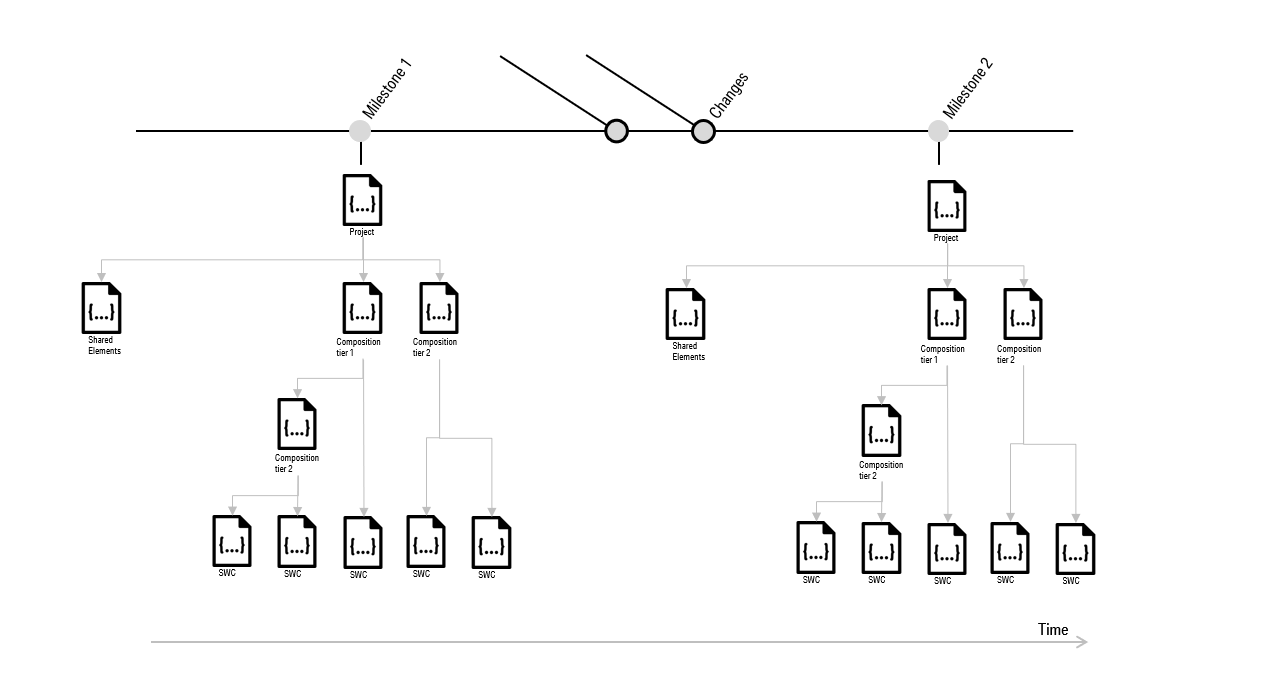
\includegraphics[width=\linewidth]{images_folder/softwarestrucutre.png}
    \caption{Software structure}
    \label{fig:SWsTR}
\end{figure}
\section{Hierarchical structure and primary key decisions}
\section{MVP definition}
\subsection{Double layering the primary key - Double layer of abstraction introduced}
\section{Database integration}
\section{Piepline steps definition}
\section{Instantiation of a Jenkins job}
\subsection{Propsor information}
\subsection{BCI information}
\cleardoublepage
\end{document}